\chapter{Implementación}
Después de decidir las características de las que dispondrá \jj es necesario analizar como se implementaran estas. Por el lado de \cc tenemos que las interfaces que definen el comportamiento de las clases que contendrán a las sentencias SQL comparten muchas cosas por lo que hay que analizar adecuadamente las herencias y definición de interfaces. Elegir adecuadamente la estructura del proyecto puede hacer la diferencia entre una librería\footnote{como lo defino al final!!!!!!} mantenible y ampliable contra una pila de código difícil de entender. Así que como en el capitulo anterior analizaremos \jj por secciones  primero la sección que se encarga de manejar la conexión con la base de datos y después la que se encarga de abstraer el uso de SQL.






\section{Implementación de el envoltorio de \jj}

A few words




\section{Implementación de \cc}

Para la implementación de las especificaciones declaradas anteriormente nos encontramos con que existen algunas similitudes entre las diferentes clases definidas anteriormente, atendiendo a que cada clase representa a una de las sentencias SQL que se incluyeron en el proyecto y cada clase esta compuesta por:
\begin{itemize}
\item Variables que almacenaran los datos necesarios para la construcción de los métodos.

\item Métodos para inicializar la clase y agregar (lo que comúnmente se dice\textit{setear}), es decir poblarla con los datos necesarios para su construcción.

\item Métodos para armar la sentencia.

\end{itemize}

Se puede hacer una distinción en como funcionan las funciones, o mas bien como responde JDBC cuando procesa determinada sentencia SQL. Por un lado están aquellos que solo necesitan reportar la cantidad de filas afectadas por la sentencia después están aquellos que necesitan devolver información después de ejecutada la sentencia, estas ultimas sentencias son precisamente las que realizan consultas sobre la base de datos siendo las sentencias \verb=SELECT= las únicas que hacen esto. Por otro lado las sentencias \verb=UPDATE=, \verb=INSERT= y \verb=DELETE= solo precisan reportar la cantidad de columnas que fueron afectadas por la consulta, en cambio las sentencias \verb=ALTER TABLE= y \verb=CREATE TABLE= que sirven para modificar las tablas (son parte del DDL de SQL) no afectan directamente a las columnas pero por convención se tomo que JDBC devuelva 0 como numero de columnas afectadas por lo que en este caso se las agrupara en el mismo conjunto. Para que \jj pueda hacer distinción de estos dos tipos de consultas se utilizaron dos interfaces las cuales pueden ser tomadas como tipos genéricos, la \figpage{fig:crossdb-base} muestra estas interfaces.\\

\begin{figure}
  \centering
    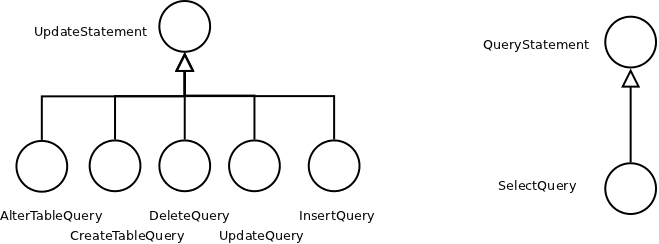
\includegraphics[width=0.5\textwidth]{figuras/crossdb-base.png}
  \caption{Interfaces base para los tipos de sentencia}
  \label{fig:crossdb-base}
\end{figure}

De este modo estamos usando las interfaces como un tipo genérico, es decir si en la firma de cualquier método declaramos algo similar a lo siguiente \verb=metodoA(UpdateStatement param)= el parámetro param podrá ser cualquier clase que implemente directa o indirectamente mediante herencia la interfase \verb=UpdateStatement=, en nuestro caso estas no se implementara directamente esa interfaz sino que se crearan otras interfaces "hijas" de \verb=UpdateStatement=.\\

\begin{figure}
  \centering
    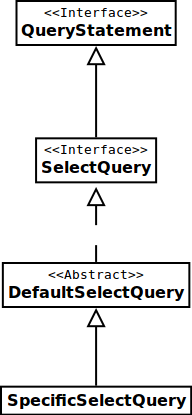
\includegraphics[width=0.2\textwidth]{figuras/crossdb-query.png}
  \caption{Mi Figura}
  \label{fig:query}
\end{figure}

En la \figpage{fig:query} tenemos una vista mas completa de como se compone la estructura de estos tipos, es la mas simple pues solo tiene una clase hija la única que sirve para hacer consultas sobre la base de datos la sentencia \verb=SELECT=. Como ya dijimos la primer interface sirve para distinguir a nivel mas genérico el tipo de sentencia SQL que se esta tratando, la interfase hija directa de \verb=QueryStatement= si ya define un comportamiento especifico para las funciones de las sentencias \verb=SELECT=. La clase abstracta \verb=DefaultSelectQuery= brinda una implementación base para los métodos definidos en \verb=SelectQuery=, para comprender por que hago esto es necesario recordar que la clase que represente una sentencia contiene toda la información necesaria para generar una sentencia valida y esta información es la misma que se precisa para cualquier sentencia SQL de un \dd en concreto (además ya definimos una sintaxis que es totalmente soportada) la diferencia esta en el modo que se escriben las sentencias, la sintaxis, por ello el único método que debería ser especifico a un \dd seria aquel que esta encargado de armar la sentencia. Después de la clase abstracta si por fin tenemos implementaciones especificas para un motor en particular \verb=SpecificSelectQuery=, de estas clases tendremos tantas como motores estén soportados por el proyecto.\\

\begin{figure}
  \centering
    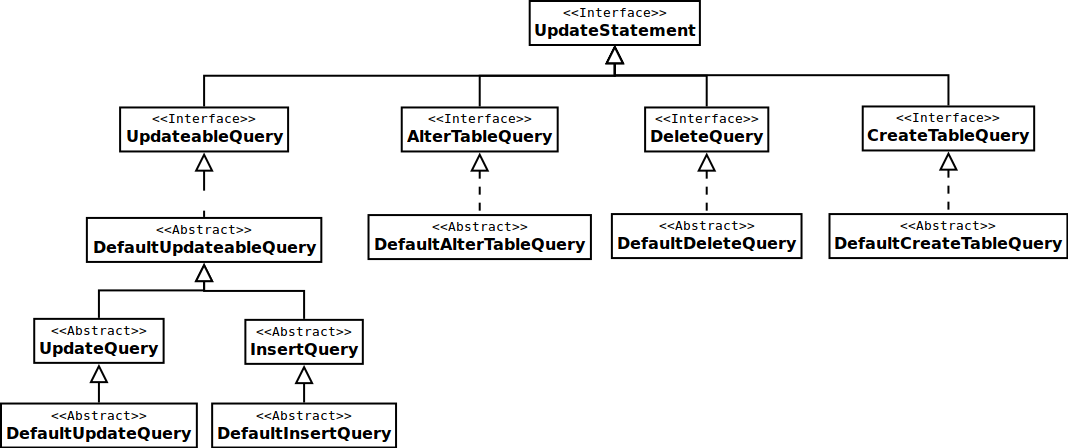
\includegraphics[width=\textwidth]{figuras/crossdb-update.png}
  \caption{Estructura de}
  \label{fig:update}
\end{figure}

En la \figpage{fig:update} tenemos una descripción de como se componen los otros tipos de sentencias, esta es algo mas elaborada, como antes la primer interfaz, funciona como tipo genérico, en las clases hijas de esta vemos algo parecido al caso de \verb=QueryStatement= salvo por la interfaz \verb=UpdateableQuery= que agrupa comportamiento común a \verb=Updatequery= e \verb=InsertQuery=, también se brinda un comportamiento predeterminado mediante \verb=DefaultUpdateStatement= pero el cual al brindar una implementación base tiene que ser a la fuerza una clase abstracta\footnote{Una clase abstracta se puede ver como una interfaz que fuerza la implementación de su comportamiento} así que las clases que definen el comportamiento especifico de \verb=UpdateQuery= e \verb=InsertQuery= son clases abstractas y no interfaces, pero el resultado es el mismo. A continuación un análisis mas detallado de como se componen las interfaces finales y las clases que las implementan además de una vista a su implementación y las clases que sirven como componente de las principales.

\subsection{Clases extras}\label{sec:extras}
Para la adecuada implementación de las clases que representaran a las sentencias seleccionadas en el capitulo \ref{cap:disenio} es necesario crear algunas clases extras que brindan funcionalidades comunes a varias clases o bien funcionalidades extras no propias de duchas clases, a continuación un listado de aquellas mas relevantes:
\begin{enumerate}

\item \verb=Column= Representa una columna de una tabla para ello posee atributos tales como nombre de columna, banderas que indican si es clave primaria o foranea y todos los demás atributos que sirven para definir la columna en una sentencia \verb=CREATE TABLE=. Entre sus métodos no se incluye ninguno que sirva para convertir la columna en una cadena  de texto que sirva para definirla en una sentencia SQL pues a pesar de que la sintaxis de la definición de columna no varia, salvo por los tipos de datos, si varia el uso sobre ella pues la sentencia \verb=ALTER TABLE= también puede definir columnas en su sintaxis pero con ciertas restricciones como se ve en la sección \ref{sec:altertable} y para evitar confusiones cada clase (clase que represente una sentencia) que haga uso de un objeto columna deberá implementar las restricciones sobre la construcción de la sentencia ignorando los atributos que no use. 

\item \verb=DataTypes= Es una clase abstracta que define el comportamiento de las clases que serán encargadas de mapear los tipos de datos genéricos usados en \cc a los tipos de datos concretos para cada motor, la clase define un solo método \verb=getAsString(Column col)= que a partir de un objeto \verb=Column= tomado como parámetro devuelve una cadena de texto que contiene el tipo de datos especifico. Aparte se tiene un método abstracto que tiene por objetivo concreto mapear el tipo de dato genérico con el tipo especifico.  

\item \verb=Formatter=

\item \verb=WhereCondition= Es una clase muy simple que tiene por objetivo la representación de las condiciones $ x = y $ que se usan dentro de una cláusula WHERE. La clase puede contener los nombres de las tablas a comparar, si es que se comparan valores de mas de una tabla, los nombres de los campos a comparar y (de haber) algún valor contra el que comparar.

\item \verb=WhereClause=  Representa una cláusula \verb=WHERE= como por ejemplo \verb|WHERE x = y | , la cláusula where esta formada por diferentes condiciones del tipo \verb=WhereCondition= e incluir cláusulas \verb=WhereClause= anidadas como por ejemplo \verb|WHERE (x = y AND (x=z OR x=b))|. Entonces cada conjunto de paréntesis puede ser visto como una cláusula \verb=WHERE=, y básicamente podemos ver a \verb=WhereClause= como una lista de condiciones y/o cláusulas \verb=WHERE=.

\item \verb=Join= Básicamente representa las condiciones de \verb=JOIN= para las sentencias \verb=SELECT=.

\item Clases constructoras de Objetos (\textit{Factories})

\end{enumerate}


\subsection{Implementación de AlterTableQuery}
Todas las interfaces menos \verb=SelectQuery= descienden de \verb=UpdateStatement=, esta es una interfaz que no define comportamiento alguno solo sirve para categorizar las interfaces hijas en cuanto a pertenencia o no a el grupo de las sentencias que no devuelven datos de la base de datos si no sobre la base de datos, su implementación a continuación:

\begin{lstlisting}[title=interfaz UpdateStatement]
package com.crossdb.sql;

public interface UpdateStatement {

}
\end{lstlisting}

La interfaz \verb=AlterTable= si ya define el comportamiento para las clases hijas de la misma que servirán para armar las sentencias \verb=ALTER TABLE=, al ser la sintaxis soportada muy limitada la interfaz es bastante simple. Se definen los métodos necesarios para poblar la sentencia de datos y despúes armarla. La función que devuelve la sentencia propiamente dicha sera la típica \verb=toString()= pero redefinida para que devuelva adecuadamente la sentencia SQL adecuada. 

\begin{lstlisting}[title=interfaz AlterTableQuery]
package com.crossdb.sql;

public interface AlterTableQuery extends UpdateStatement{
	
	void setTable(String table);
	
	void addColumn(Column c);
	
	void newTableName(String table);
}
\end{lstlisting}
Hay algunas cosas a tener presentes por ejemplo el método \verb=addColumn(Column)= utiliza la clase \verb=Column= que representa una columna tal como se definió en \ref{sec:extras}. Además las funciones \verb=addColumn(Column)= y \verb=newTableName(String)= que respectivamente sirven para añadir columnas a la tabla y renombrar la misma son mutuamente excluyentes en el sentido que una sentencia solo puede realizar unas de las acciones previamente nombradas a la vez, por lo que si en un mismo objeto se llamase a las dos funciones solo tendrá efecto la ultima en ser llamada.\\

En cuanto a la implementación base \verb=DefaultALterTableQuery= hay poco que comentar pues únicamente agrega los atributos necesarios para implementar las funciones definidas en \verb=AlterTableQuery=, las hijas de esta clase ya serán especificas para un \dd concreto, en nuestra implementación contamos con tres a saber:
\begin{itemize}
\item \verb=MySQLAlterTableQuery=
\item \verb=SQLiteAlterTableQuery=
\item \verb=PostgreSQLAlterTableQuery=
\end{itemize}
Cuya única misión es implementar, o re-implementar si se quiere, el método \verb=toString()= que entregara la sentencia SQL en forma de cadena de texto dentro de un objeto String.




\subsection{Implementación de DeleteQuery}
La sintaxis soportada para \verb=DeleteQuery= es muy limitada por lo que es posible observar casi todo el código de la Interfaz principal para estas sentencias:

\begin{lstlisting}[title=código interfaz QueryStatement]
package com.crossdb.sql;

public interface DeleteQuery extends UpdateStatement{

	void setTable(String table);

	void addWhereCondition(String x, int comparison, String y);

	void addWhereCondition(String x, int comparison, int y);

	void addWhereCondition(String x, int comparison, java.util.Date y);

	void addWhereCondition(String and_or, String x, int comparison, String y);

	void addWhereCondition(String and_or, String x, int comparison, int y);

	void addWhereCondition(String and_or, String x, int comparison,
			java.util.Date y);

	void addWhereCondition(WhereCondition cond);

	void addWhereClause(WhereClause wc);

	void addWhereString(String x, int comparison, String y);

	void addWhereString(String and_or, String x, int comparison, String y);

	void addWhereNotNull(String col);

	void addWhereNotNull(String and_or, String col);

	void addWhereIsNull(String col);

	void addWhereIsNull(String and_or, String col);
	new

}
\end{lstlisting}



\subsection{Implementación de UpdateQuery e InsertQuery}




\subsection{Implementación de CreateTableQuery}




\subsection{Implementación de selectQuery}

Esta interfaz es la única que desciende de la interfaz padre \verb=QueryStatement= la cual podemos ver en su totalidad ya que se trata de una interfaz muy simple:

\begin{lstlisting}[title=código interfaz QueryStatement]
package com.crossdb.sql;

public interface QueryStatement {

}
\end{lstlisting}

Como ya se dijo no necesita definir ningún comportamiento, salvo por la pertenencia a un grupo que es en este caso la de el tipo de sentencias que ejecutan consultas sobre la base de datos. La interfaz hija si ya define comportamientos específicos que servirán para poblar de datos y armar las sentencias \verb=SELECT= las métodos mas importantes de su implementación la podemos ver a continuación:

\begin{lstlisting}[title=código interfaz UpdateStatement]
package com.crossdb.sql;

import java.util.Date;
import com.crossdb.sql.optimization.OptimizationHint;

public interface SelectQuery extends QueryStatement {

	void addColumn(String column);

	void addFunctionColumn(String function, String column);

	void sumColumn(String column);

	void countColumn(String column);

	void countColumn(String table, String column);

	void averageColumn(String column);

	void averageColumn(String table, String column);

	void minColumn(String column);

	void minColumn(String table, String column);

	void maxColumn(String column);

	void maxColumn(String table, String column);

	void addTable(String table);

	void addTable(int joinType, String table);

	void addTable(int join_type, String table, WhereCondition cond);

	void addTable(Join join);

	void addWhereCondition(String x, int comparison, String y);

	void addWhereCondition(String x, int comparison, int y);

	void addWhereCondition(String x, int comparison, long y);

	void addWhereCondition(String x, int comparison, Date y);

	void addWhereCondition(String and_or, String x, int comparison, String y);

	void addWhereCondition(String and_or, String x, int comparison, int y);

	void addWhereCondition(String and_or, String x, int comparison, long y);

	void addWhereCondition(String and_or, String x, int comparison, Date y);

	void addWhereString(String x, int comparison, String y);

	void addWhereString(String and_or, String x, int comparison, String y);

	void addWhereCondition(WhereCondition cond);

	void addWhereClause(IWhereClause wc);

	void addOrderBy(String order_by);

	void addGroupBy(String group_by);

	void union(SelectQuery sq);

	void setDistinct(boolean distinct);

	void setLimit(int offset, int rowCount);

}
\end{lstlisting}
